With our implementation we want to answer the following question:
\begin{quote}
  ``Given some differential characteristic, is this characteristic valid?''
\end{quote}
Equivalently is there any boolean assignment within both evaluation instances such that the applied function of the hash algorithm matches the result and the bit conditions do correspond. This question was already raised in section~\ref{sec:diffchar-examples}. This is the same question stated as main difficulty for the attack of SHA-2~\cite[293]{Cry07} when trying to apply automated search.

\section{General architecture}
\label{sec:architecture}
%
In the following we discuss various architectures to evaluate the validity of differential characteristics. We try to achieve the best performance for this task within \nltool{}'s automated search.

\subsection{Hash algorithm specification and truth table}
%
At the very beginning we specify a hash algorithm. This specification contains the elementary operations. We consider some simple hash algorithm applying the SHA-2 Sigma operation consisting of XOR operations:
\lstset{language={C++},caption={A very basic hash algorithm specification},label={lst:sigma}}
\begin{lstlisting}
  satstep->Add<SatGenerator<XOR3>>(
    a->Rotr(1), a->Rotr(2), a->Rotr(3), b
  );
\end{lstlisting}

Here \texttt{satstep} is the computational unit which uses the SAT solver to report whether a given differential characteristic is valid or not. \texttt{SatGenerator} is a wrapper which takes a conventional implementation like XOR of 3-digit values (manipulating values in the main memory) and creates a SAT solver equivalent for it. This is done by evaluating the truth table of the values after application of one such operation. \texttt{a} and \texttt{b} are differential words. \texttt{Rotr} rotates the given values to the right. Its number of rotations is defined in the parameter. By definition of \texttt{XOR3}, the fourth value ($\texttt{b}$) represents the result.

Every operation statically knows how many parameter it takes. The XOR3 operation takes three input parameters and one output parameter. The truth table is created once for every operation and determines which output value is generated for the given input. As such the truth table evaluation is a bottleneck in the framework due to its exponential behavior. However, a static implementation of the operation which directly adds the clauses can also be provided (thus omitting the \texttt{SatGenerator} wrapper).

Using a command line parameter \texttt{nltool} gets to know which hash algorithm to take. At this point in time, it is going to know which parameters (and their relation) are used for this hash algorithm, but not their actual values. At the same time an instance of the SAT solver is instantiated to be used later on.

The following properties are given for the primitive functions and the hash algorithm:
\begin{itemize}
  \item Any pure function using integers as arguments can be transformed into a SAT equivalent.
  \item A truth table is used exploiting exponential behavior, but this truth table generation is only run once. In a different implementation it might also run at compile time.
  \item \texttt{satstep} describes a computational unit of any scale thus allowing to combine elementary operations to advanced algebraic operations, hash algorithm rounds or even whole hash algorithms.
\end{itemize}

\subsection{Clause introduction}
\label{sec:clause-introduction}
%
Constraints to the solution of the SAT solver will be introduced in two places. The actual clauses are defined by some encoding explained in section~\ref{sec:three-approaches}:
\begin{itemize}
  \item Every bit condition is represented by a set of clauses. In our implementation we introduced a \texttt{SatCondition} object which takes a bit condition as parameter and the \texttt{addClauses} method will add all corresponding clauses to the SAT solver.
  \item The hash algorithm defines which functions are applied. This function is analyzed using a truth table and the corresponding clauses are generated.
\end{itemize}

\subsection{Structure of encodings}
\label{sec:encoding-structure}
%
A distinction of the \emph{Init} and \emph{Update} step was already defined in section~\ref{sec:nltool}. Those steps are split into several substeps in all encodings:
\begin{enumerate}
  \item Initialization
    \begin{enumerate}
      \item Detect Overlapping bits: Sometimes bit conditions are reused within a hash algorithm. For example one differential word is the rotated version of another differential word as in SHA-2 Sigma. In such a case the two bit conditions connected through rotation must be equivalent. In this step the reuse of bit conditions is detected. See section~\ref{sec:automated-search} for a more detailed discussion of overlapping bits.
      \item Introduce new bit conditions: Introduce a new \texttt{SatCondition} object (SAT equivalent of a bit condition) for every bit condition.
      \item Setup encoding: For assumption-based encoding, \textbf{clauses} are added here (the ones that must be added \textbf{for every \texttt{SatCondition} object}). Request the required boolean variables for each \texttt{SatCondition} object.
      \item Apply function to bitslices: Elementary functions in \nltool{} are defined per bitslice. In this step the function is applied successively to every bitslice \textbf{adding clauses specific for the function}.
    \end{enumerate}
  \item Update BitCondition
    \begin{enumerate}
      \item Set bit condition value: Take the bit condition value and infer the corresponding \textbf{clauses or assumptions} depending on the encoding.
      \item Run SAT solver: Invoke the SAT solver and return its result as result.
    \end{enumerate}
\end{enumerate}

\section{Three approaches}
\label{sec:three-approaches}

\subsection{Approach \#1: Simple evaluation}
\label{sec:encoding:simple-evaluation}
%
The simple evaluation approach uses 2 boolean variables per bit condition. This corresponds to one bit per evaluation instance.

\subsubsection{Algorithm}
\label{sec:simple-evaluation-algorithm}
%
\begin{description}
  \item[Initialization] Overlapping bits and the number of bit conditions are known.
    \begin{description}
      \item[Detect Overlapping Bits] Iterate over all bit conditions and recognize which bit conditions are overlapping (see section~\ref{sec:automated-search}). Store all their indices for future reference.
      \item[Introduce new bit conditions] Introduce a new \texttt{SatCondition} object for every bit condition that will be used. A bit condition gets skipped, if this is not the first reference to an overlapping bit.
      \item[Setup Encoding] $2$ boolean variables per bit condition are requested from the SAT solver.
      \item[Apply function to bitslices] Add all clauses which result from the function definition applied to this differential characteristic.
    \end{description}
  \item[Update BitCondition] The values of the bit conditions are known.
    \begin{description}
      \item[Set bit condition value] The clauses resulting from the bit condition value are added. These clauses were already discussed in the paper ``Linear propagation in Efficient Guess-and-Determine Attacks''~\cite[6]{Cry16} and illustrated in Table~\ref{tab:simple-eval-clauses} again. Some are them are written as XOR clauses, which are only supported by \cmsat{}. If the SAT solver does not provide XOR clauses, the SAT solver abstraction discussed in section~\ref{sec:satsolver-abstraction} provides a corresponding encoding to CNF.
      \item[Run SAT solver] If the SAT solver returns satisfiability as result, the differential characteristic is valid.
    \end{description}
\end{description}

\begin{table}[p]
  \begin{center}
    \begin{tabular}{cl}
      bit condition  & conjunctive normal form \\
    \hline
      \bc{\#}        & $(z) \land (\neg z)$ \\
      \bc{0}         & $(\neg z) \land (\neg z^*)$ \\
      \bc{u}         & $(z) \land (\neg z^*)$ \\
      \bc{3}         & $(\neg z^*)$ \\
      \bc{n}         & $(\neg z) \land (z^*)$ \\
      \bc{5}         & $(\neg z)$ \\
      \bc{x}         & $(\neg z \lor \neg z^*) \land (z \lor z^*)$ \\
                     & or as XOR clause: $(z \oplus z^*)$ \\
      \bc{7}         & $(\neg z \lor \neg z^*)$ \\
      \bc{1}         & $(z) \land (z^*)$ \\
      \bc{-}         & $(\neg z \lor z^*) \land (z \lor \neg z^*)$ \\
                     & or as XOR clause: $\neg (z \oplus z^*)$ \\
      \bc{A}         & $(z)$ \\
      \bc{B}         & $(z \lor \neg z^*)$ \\
      \bc{C}         & $(z^*)$ \\
      \bc{D}         & $(\neg z \lor z^*)$ \\
      \bc{E}         & $(z \lor z^*)$ \\
      \bc{?}         & 
    \end{tabular}
    \caption[Simple Evaluation clauses]{
        Simple Evaluation clauses added for a bit condition.
        A bit condition corresponds to two boolean variables $z$ and $z^*$.
    }
    \label{tab:simple-eval-clauses}
  \end{center}
\end{table}

\subsubsection{Discussion}
\label{sec:simple-evaluation-discussion}
%
This approach was implemented first, but has a major problem: Assuming the evaluated differential characteristic is valid, a more restrictive bit condition will be used by the automated search at one position. However for the next iteration the SAT solver has to be destroyed and the configuration must be built up again. This takes a long time. We can use the fact that the Initialization step stays the same, but the Update BitCondition step is different. And so we want to use an approach which runs the Initialization step only once and the Update BitCondition is run on every search iteration.

This approach was not put into practice for the automated search and so no performance statistics are available here.

For the Update BitCondition step we are going to use SAT solver assumption. These are assignments to boolean variables which will be discarded after one run of the SAT solver without the loss of the clauses (as discussed in section~\ref{sec:satsolvers-assumptions}). Assignments are not as powerful as clauses and so the encoding has to be designed in such a way that we can use assignments to define the value of a bit condition.

\subsection{Approach \#2: Activation literals}
\label{sec:encoding:activation-literals}
%
This approach uses the concept of \emph{activation literals}. Even though there is no explicit definition of activation literals given in prior work, the concept is used recurrently by the SAT community. One example of such is given in a paper by Niklas Een, Alan Mishchenko and Nina Amla~\cite{Sat30}.

Given a clause $c$ we introduce an activation literal $a$ to activate or deactivate this clause. Activation means that this clause becomes part of the result of the \gls{cnf}. Deactivation means that this
clause becomes true anyway and therefore is not relevant for the result. $a$ is used to distinguish the (de)activation cases.

These requirements can be implemented using an implication.
\[
  a \implies b
\]

\subsubsection{Search with activation literals}
\label{sec:activation-literals-search}
%
To evaluate a path in the search tree a generalization of activation literals is required. We apply activation literals to sets of clauses.

Given sets of sets of clauses $S_1, S_2, S_3, \ldots, S_n$ representing nodes of a search tree, evaluate which path of this tree is satisfiable. One node is satisfiable, if all clauses of this node are satisfied. Assume a binary tree of depth 2 with $S_2$ and $S_3$ as children of $S_1$ and $S_4$ and $S_5$ as children of $S_2$ and $S_6$ and $S_7$ as children of $S_3$. The first path is given as the union of $S_1$, $S_2$ and $S_4$: $S_1 \land S_2 \land S_4$. If this path is not satisfiable, replace $S_4$ with $S_2$'s other child $S_5$ giving $S_1 \land S_2 \land S_5$. If this fails again we replace $S_2$ with $S_3$ giving us $S_1 \land S_3 \land S_6$ and $S_1 \land S_3 \land S_7$. With this concept we can evaluate any path of the tree after evaluation which clauses are part of which node.

\begin{figure}[h]
  \begin{center}
    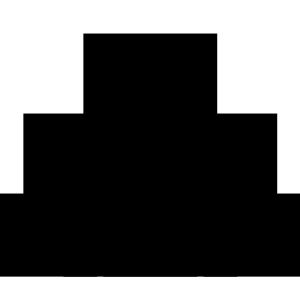
\includegraphics{img/searchtree.pdf}
    \caption{Binary search tree with sets of sets of clauses as nodes.}
    \label{fig:bintree_clauses}
  \end{center}
\end{figure}

This tree traversal can be implemented using activation literals and SAT solver assumption techniques.

If we want to evaluate the path $S_1 \land S_2 \land S_4$, we introduce a new activation literal $a_i$ for each set $S_i$ and use implication to (de)activate the clause:
%
\[
  (a_1 \implies S_1) \land (a_2 \implies S_2) \land (a_4 \implies S_4)
\]

Because each node itself is a conjunctive normal form, a set $S_i$ is the conjunction of its clauses giving us:
%
\[
  (a_1 \implies (c_1 \land c_2 \land c_3 \land \ldots)) \land
    (a_2 \implies (c_{10} \land c_{11} \land c_{12} \land \ldots)) \land
    (a_3 \implies (c_{20} \land c_{21} \land c_{22} \land \ldots)) \land
    \ldots
\]

This can be transformed to conjunctive normal form by resolving the clauses with the law of distributivity. In real-world implementations activation literals are represented as \emph{assumptions} in SAT solvers
to be able to drop their value for evaluation of the next search path (assumptions are described in section~\ref{sec:satsolvers-assumptions}).

For example the conjunctive normal form with boolean variables $v_1$ to $v_8$
%
\[
  (v_1 \lor \neg v_2) \land (\neg v_3 \lor \neg v_4 \lor v_5) \land
    (v_6 \lor v_7 \lor v_8)
\]

with activation literals $a_1$ to $a_3$
\[
  (a_1 \implies (v_1 \lor \neg v_2)) \land
    (a_2 \implies (\neg v_3 \lor \neg v_4 \lor v_5)) \land
    (a_3 \implies (v_6 \lor v_7 \lor v_8))
\]

resolved with the law of distributivity
\[
  (\neg a_1 \lor v_1 \lor \neg v_2) \land
    (\neg a_2 \lor \neg v_3 \lor \neg v_4 \lor v_5) \land
    (\neg a_3 \lor v_6 \lor v_7 \lor v_8)
\]

gives us a boolean expression in CNF.

\subsubsection{Algorithm}
\label{sec:activation-literals-algorithm}
%
\begin{description}
  \item[Initialization] Overlapping bits and the number of bit conditions are known.
    \begin{description}
      \item[Detect Overlapping Bits] Iterate over all bit conditions and store overlapping bit conditions.
      \item[Introduce new bit conditions] Introduce a new \texttt{SatCondition} object for every bit condition that will be used. A bit condition gets skipped, if this is not the first reference to an overlapping bit.
      \item[Setup Encoding] $7$ boolean variables per bit condition are requested from the SAT solver. The clauses given in Table~\ref{tab:simple-eval-clauses} are added.
      \item[Apply function to bitslices] Add all clauses which result from the function definition applied to this differential characteristic.
    \end{description}
  \item[Update BitCondition] The values of the bit conditions are known.
    \begin{description}
      \item[Set bit condition value] The assumptions resulting from the bit condition value are created. They are given in Table~\ref{tab:simple-eval-clauses}.
      \item[Run SAT solver] If the SAT solver returns satisfiability as result, the differential characteristic is valid.
    \end{description}
\end{description}

\begin{table}[p]
  \begin{center}
    \begin{tabular}{cll}
      bit condition  & Setup Encoding (\gls{cnf})                        & Set bit condition value (assumptions) \\
    \hline
      \bc{\#}        & $(\neg a_1 \lor z) \land (\neg a_1 \lor \neg z)$  & $a_1 = 1$ \\
      \bc{0}         &                                                   & $z = 0, z^* = 0$ \\
      \bc{u}         &                                                   & $z = 1, z^* = 0$ \\
      \bc{3}         &                                                   & $z^* = 0$ \\
      \bc{n}         &                                                   & $z = 0, z^* = 1$ \\
      \bc{5}         &                                                   & $z = 0$ \\
      \bc{x}         &                                                   & $a_2 = 1, a_5 = 1$ \\
      \bc{7}         & $(\neg a_2 \lor \neg z \lor \neg z^*)$            & $a_2 = 1$ \\
      \bc{1}         &                                                   & $z = 1, z^* = 1$ \\
      \bc{-}         &                                                   & $a_3 = 1, a_4 = 1$ \\
      \bc{A}         &                                                   & $z = 1$ \\
      \bc{B}         & $(\neg a_3 \lor z \lor \neg z^*)$                 & $a_3 = 1$ \\
      \bc{C}         &                                                   & $z^* = 1$ \\
      \bc{D}         & $(\neg a_4 \lor \neg z \lor z^*)$                 & $a_4 = 1$ \\
      \bc{E}         & $(\neg a_5 \lor z \lor z^*)$                      & $a_5 = 1$ \\
      \bc{?}         &                                                   &
    \end{tabular}
    \caption[Activation literals clauses and assumptions]{
        Activation literals clauses and assumptions.
        Be aware that all activation literals $a_i$ must be set to false,
        if not stated otherwise.
    }
    \label{tab:simple-eval-clauses}
  \end{center}
\end{table}

\subsubsection{Discussion}
\label{sec:activation-literals-discussion}
%
The number of activation literals is linear to the number of nodes within the search tree. Every node represents one of sixteen possible bit conditions. However not all bit conditions have to be encoded using activation literals\footnote{This approach would obviously possible but less efficient}.

The bit conditions \bc{\#}, \bc{0}, \bc{u}, \bc{3}, \bc{n}, \bc{5}, \bc{1}, \bc{A}, \bc{C} and \bc{?} can directly be represented by assignments. The $6$ bit conditions \bc{x}, \bc{7}, \bc{-}, \bc{B}, \bc{D} and \bc{E} use the $\lor$ operator which has to be designed by explicit clauses.

For one additional bit condition we need $6$ clauses, $5.6875$ assumptions ($21$ assumptions from the right column in Table~\ref{tab:simple-eval-clauses} and $70$ activation literals set to false divided by $16$ bit conditions) and $7$ variables in average. Due to the high number of assumptions it was estimated that another approach would be more successful and no implementation is provided. No statistics are available. But this estimation is biased and requires further investigation in follow-up scientific work.

\subsection{Approach \#3: Assumption-based encodings}
\label{sec:encoding:assumption-encodings}
%
Like the activation literals approach in section~\ref{sec:encoding:activation-literals}, these approaches uses assumption to enable automated search. They do not use activation literals and only focus on efficient usage of assumptions. Three different approaches are taken which vary in the number of variables, clauses and assumptions.

\subsection{Exhaustive Encoding}
\label{sec:encoding:exhaustive}
%
The Exhaustive encoding consists of $17$ boolean variables per bit condition. Exhaustive refers to the large number of boolean variables. Each differential state gets its own assumption variable.

\subsubsection{Algorithm}
\label{sec:exhaustive-algorithm}
%
\begin{description}
  \item[Initialization] Overlapping bits and the number of bit conditions are known.
    \begin{description}
      \item[Detect Overlapping Bits] Iterate over all bit conditions and store overlapping bit conditions.
      \item[Introduce new bit conditions] Introduce a new \texttt{SatCondition} object for every bit condition that will be used. A bit condition gets skipped, if this is not the first reference to an overlapping bit.
      \item[Setup Encoding] $17$ boolean variables per bit condition are requested from the SAT solver. The clauses given below this algorithm are added.
      \item[Apply function to bitslices] Add all clauses which result from the function definition applied to this differential characteristic.
    \end{description}
  \item[Update BitCondition] The values of the bit conditions are known.
    \begin{description}
      \item[Set bit condition value] Given a bit condition $T$, the corresponding assumption $z_T$ is set to true.
      \item[Run SAT solver] If the SAT solver returns satisfiability as result, the differential characteristic is valid.
    \end{description}
\end{description}

\begin{align*}
  z_\# & = \neg z_\#                          & \text{1 XOR clause or 2 CNF clauses} \\
  z_0  & = \neg z \land \neg z^*              & \text{3 CNF clauses} \\
  z_u  & = z \land z^*                        & \text{3 CNF clauses} \\
  z_3  & = \neg z^*                           & \text{1 XOR clause or 2 CNF clauses} \\
  z_n  & = \neg z^* \land z^*                 & \text{3 CNF clauses} \\
  z_5  & = \neg z                             & \text{1 XOR clause or 2 CNF clauses} \\
  z_X  & = z \oplus z^*                       & \text{4 CNF clauses} \\
  z_7  & = \neg z \lor \neg z^*               & \text{4 CNF clauses} \\
  z_1  & = z \land z^*                        & \text{3 CNF clauses} \\
  z_-  & = \neg(z \oplus z^*)                 & \text{1 XOR clauses or 4 CNF clauses} \\
  z_A  & = z                                  & \text{1 XOR clauses or 2 CNF clauses} \\
  z_B  & = \neg((z \land z^*) \oplus z^*)     & \text{4 CNF clauses} \\
  z_C  & = z^*                                & \text{1 XOR clause or 2 CNF clauses} \\
  z_D  & = \neg(z \land z^* \lor z)           & \text{4 CNF clauses} \\
  z_E  & = ((z\land z^*) \oplus z \oplus z^*) & \text{4 CNF clauses} \\
\end{align*}

The bit condition $?$ is skipped, because it does not constrain the boolean system in any way.

\subsubsection{Discussion}
\label{sec:exhaustive-discussion}
%
For this encoding obviously some reductions can be applied if one bit condition is a superset of another one (as can be seen in the lattice of Figure~\ref{fig:bitconditions-lattice}). Those reductions have been applied in the following encodings. Because this encoding has an extraordinary high number of variables, we assume that this encoding will not perform good in any case. Because no implementation was provided, no statistics are available.

\subsection{Reduced Encoding}
\label{sec:encoding:reduced-encoding}
%
The following approach was initially proposed by Martin Schläffer. It takes $9$ variables for each bit condition.

\subsubsection{Algorithm}
\label{sec:reduced-encoding-algorithm}
%
The 9 variables are denoted as $z, z^*, z_A, z_B, z_C, z_D, z_E, z_x$ and $z_1$.
%
\begin{description}
  \item[Initialization] Overlapping bits and the number of bit conditions are known.
    \begin{description}
      \item[Detect Overlapping Bits] Iterate over all bit conditions and store overlapping bit conditions.
      \item[Introduce new bit conditions] Introduce a new \texttt{SatCondition} object for every bit condition that will be used. A bit condition gets skipped, if this is not the first reference to an overlapping bit.
      \item[Setup Encoding] $9$ boolean variables per bit condition are requested from the SAT solver. The clauses given below this algorithm are added.
      \item[Apply function to bitslices] Add all clauses which result from the function definition applied to this differential characteristic.
    \end{description}
  \item[Update BitCondition] The values of the bit conditions are known.
    \begin{description}
      \item[Set bit condition value] The assumptions resulting from the bit condition value are created. They are given in Table~\ref{tab:reduced-encoding-assumptions}.
      \item[Run SAT solver] If the SAT solver returns satisfiability as result, the differential characteristic is valid.
    \end{description}
\end{description}

In the Setup Encoding step the following relations are defined for the variables:
\begin{align*}
  z_A & = z_1                   & \text{1 XOR clause or 2 CNF clauses} \\
  z_B & = z_1 \lor \neg z_1^*   & \text{3 CNF clauses} \\
  z_C & = z^*                   & \text{1 XOR clause or 2 CNF clauses} \\
  z_D & = \neg z \lor z^*       & \text{3 CNF clauses} \\
  z_E & = z \lor z^*            & \text{3 CNF clauses} \\
  z_X & = z \oplus z^*          & \text{1 XOR clause or 4 CNF clauses} \\
  z_1 & = z \land z^*           & \text{1 XOR clause or 3 CNF clauses} \\
\end{align*}

Recognize that $a = (b \land c)$ can be represented by 3 clauses in CNF using $(\neg a \lor c) \land (\neg a \lor b \lor \neg c) \land (a \lor \neg b \lor \neg c)$.
\begin{table}[p]
  \begin{center}
    \begin{tabular}{cll}
      bit condition  & Set bit condition value \\
    \hline
      \bc{\#}        & $z_1 = 1, z_x = 1$ \\
      \bc{0}         & $z_A = 0, z_C = 0$ \\
      \bc{u}         & $z_A = 1, z_C = 0$ \\
      \bc{3}         & $z_C = 0$ \\
      \bc{n}         & $z_A = 0, z_C = 0$ \\
      \bc{5}         & $z_A = 0$ \\
      \bc{x}         & $z_X = 1$ \\
      \bc{7}         & $z_1 = 0$ \\
      \bc{1}         & $z_1 = 1$ \\
      \bc{-}         & $z_X = 0$ \\
      \bc{A}         & $z_A = 1$ \\
      \bc{B}         & $z_B = 1$ \\
      \bc{C}         & $z_C = 1$ \\
      \bc{D}         & $z_D = 1$ \\
      \bc{E}         & $z_E = 1$ \\
      \bc{?}         & 
    \end{tabular}
    \caption{Assumptions for the Reduced encoding.}
    \label{tab:reduced-encoding-assumptions}
  \end{center}
\end{table}

\subsubsection{Discussion}
\label{sec:reduced-encoding-discussion}
%
One additional bit condition requires $9$ boolean variables, $20$ clauses and $1.25$ assumptions in average.
In our SHA-256 testcase it reached up to 177 iterations per second.

\subsection{Differential state encoding}
\label{sec:encoding:dse}
%
\subsubsection{Algorithm}
\label{sec:encoding:dse-algorithm}
%
The 4 variables are denoted as $z_A, z_B, z_C$ and $z_D$. They exactly correspond to one of the cases $\{(0, 0), (0, 1), (1, 0), (1, 1)\}$ for the bits in the evaluation instances. $z_A$ corresponds to \bc{0}, $z_B$ is the same as \bc{n}, $z_C$ is \bc{u} and $z_D$ equals to \bc{1}. We require that only one of the cases is met in the Setup Encoding represented by 7 clauses.
%
\begin{description}
  \item[Initialization] Overlapping bits and the number of bit conditions are known.
    \begin{description}
      \item[Detect Overlapping Bits] Iterate over all bit conditions and store overlapping bit conditions.
      \item[Introduce new bit conditions] Introduce a new \texttt{SatCondition} object for every bit condition that will be used. A bit condition gets skipped, if this is not the first reference to an overlapping bit.
      \item[Setup Encoding] $4$ boolean variables per bit condition are requested from the SAT solver. The clauses given below this algorithm are added.
      \item[Apply function to bitslices] Add all clauses which result from the function definition applied to this differential characteristic.
    \end{description}
  \item[Update BitCondition] The values of the bit conditions are known.
    \begin{description}
      \item[Set bit condition value] The assumptions resulting from the bit condition value are created. They are given in Table~\ref{tab:dse-assumptions}.
      \item[Run SAT solver] If the SAT solver returns satisfiability as result, the differential characteristic is valid.
    \end{description}
\end{description}

The Setup Encoding clauses can be represented by 1 XOR clause and 4 CNF clauses
\begin{alignat*}{4}
  (z_A      & \oplus    z_B & & \oplus    z_C & & \oplus    z_D & & ) \land \\
  (z_A      & \lor \neg z_B & & \lor \neg z_C & & \lor \neg z_D & & ) \land \\
  (\neg z_A & \lor      z_B & & \lor \neg z_C & & \lor \neg z_D & & ) \land \\
  (\neg z_A & \lor \neg z_B & & \lor      z_C & & \lor \neg z_D & & ) \land \\
  (\neg z_A & \lor \neg z_B)& & \lor \neg z_C & & \lor      z_D & & ) \\
\end{alignat*}

or 7 CNF clauses:
\begin{alignat*}{4}
  (z_A & \lor           z_B & & \lor z_C       & & \lor z_D)      & & \land \\
  (z_A & \lor           z_B & & \lor \neg z_C  & & \lor \neg z_D) & & \land \\
  (z_A & \lor \neg      z_B & & \lor z_C       & & \lor \neg z_D) & & \land \\
  (z_A & \lor \neg      z_B & & \lor \neg z_C) & &                & & \land \\
  (\neg z_A & \lor      z_B & & \lor z_C       & & \lor \neg z_D) & & \land \\
  (\neg z_A & \lor      z_B & & \lor \neg z_C) & &                & & \land \\
  (\neg z_A & \lor \neg z_B) & &               & &                & & \\
\end{alignat*}

\begin{table}[p]
  \begin{center}
    \begin{tabular}{cll}
      bit condition  & Set bit condition value \\
    \hline
      \bc{\#}        & $z_A = 0, z_B = 0, z_C = 0, z_D = 0$ \\
      \bc{0}         & $z_A = 1$ \\
      \bc{u}         & $z_C = 1$ \\
      \bc{3}         & $z_B = 0, z_D = 0$ \\
      \bc{n}         & $z_B = 1$ \\
      \bc{5}         & $z_C = 0, z_D = 0$ \\
      \bc{x}         & $z_A = 0, z_D = 0$ \\
      \bc{7}         & $z_D = 0$ \\
      \bc{1}         & $z_D = 1$ \\
      \bc{-}         & $z_B = 0, z_C = 0$ \\
      \bc{A}         & $z_A = 0, z_D = 0$ \\
      \bc{B}         & $z_B = 0$ \\
      \bc{C}         & $z_A = 0, z_C = 0$ \\
      \bc{D}         & $z_C = 0$ \\
      \bc{E}         & $z_A = 0$ \\
      \bc{?}         & 
    \end{tabular}
    \caption{Assumptions for the Differential State encoding.}
    \label{tab:dse-assumptions}
  \end{center}
\end{table}

\subsubsection{Discussion}
\label{sec:dse-discussion}
%
One additional bit condition requires $4$ boolean variables, $7$ clauses and $1.5$ assumptions in average. The open question is which one is worse: a high number of clauses or a high number of variables. A high number of variables might segment the search space for the SAT solver which leads to fast evaluation. In this implementation further analysis is required whether this might happen for this architecture.
